
%% bare_conf.tex
%% V1.4b
%% 2015/08/26
%% by Michael Shell
%% See:
%% http://www.michaelshell.org/
%% for current contact information.
%%
%% This is a skeleton file demonstrating the use of IEEEtran.cls
%% (requires IEEEtran.cls version 1.8b or later) with an IEEE
%% conference paper.
%%
%% Support sites:
%% http://www.michaelshell.org/tex/ieeetran/
%% http://www.ctan.org/pkg/ieeetran
%% and
%% http://www.ieee.org/

%%*************************************************************************
%% Legal Notice:
%% This code is offered as-is without any warranty either expressed or
%% implied; without even the implied warranty of MERCHANTABILITY or
%% FITNESS FOR A PARTICULAR PURPOSE! 
%% User assumes all risk.
%% In no event shall the IEEE or any contributor to this code be liable for
%% any damages or losses, including, but not limited to, incidental,
%% consequential, or any other damages, resulting from the use or misuse
%% of any information contained here.
%%
%% All comments are the opinions of their respective authors and are not
%% necessarily endorsed by the IEEE.
%%
%% This work is distributed under the LaTeX Project Public License (LPPL)
%% ( http://www.latex-project.org/ ) version 1.3, and may be freely used,
%% distributed and modified. A copy of the LPPL, version 1.3, is included
%% in the base LaTeX documentation of all distributions of LaTeX released
%% 2003/12/01 or later.
%% Retain all contribution notices and credits.
%% ** Modified files should be clearly indicated as such, including  **
%% ** renaming them and changing author support contact information. **
%%*************************************************************************


% *** Authors should verify (and, if needed, correct) their LaTeX system  ***
% *** with the testflow diagnostic prior to trusting their LaTeX platform ***
% *** with production work. The IEEE's font choices and paper sizes can   ***
% *** trigger bugs that do not appear when using other class files.       ***                          ***
% The testflow support page is at:
% http://www.michaelshell.org/tex/testflow/



\documentclass[conference]{IEEEtran}
% Some Computer Society conferences also require the compsoc mode option,
% but others use the standard conference format.
%
% If IEEEtran.cls has not been installed into the LaTeX system files,
% manually specify the path to it like:
% \documentclass[conference]{../sty/IEEEtran}





% Some very useful LaTeX packages include:
% (uncomment the ones you want to load)


% *** MISC UTILITY PACKAGES ***
%
%\usepackage{ifpdf}
% Heiko Oberdiek's ifpdf.sty is very useful if you need conditional
% compilation based on whether the output is pdf or dvi.
% usage:
% \ifpdf
%   % pdf code
% \else
%   % dvi code
% \fi
% The latest version of ifpdf.sty can be obtained from:
% http://www.ctan.org/pkg/ifpdf
% Also, note that IEEEtran.cls V1.7 and later provides a builtin
% \ifCLASSINFOpdf conditional that works the same way.
% When switching from latex to pdflatex and vice-versa, the compiler may
% have to be run twice to clear warning/error messages.






% *** CITATION PACKAGES ***
%
\usepackage{cite}
% cite.sty was written by Donald Arseneau
% V1.6 and later of IEEEtran pre-defines the format of the cite.sty package
% \cite{} output to follow that of the IEEE. Loading the cite package will
% result in citation numbers being automatically sorted and properly
% "compressed/ranged". e.g., [1], [9], [2], [7], [5], [6] without using
% cite.sty will become [1], [2], [5]--[7], [9] using cite.sty. cite.sty's
% \cite will automatically add leading space, if needed. Use cite.sty's
% noadjust option (cite.sty V3.8 and later) if you want to turn this off
% such as if a citation ever needs to be enclosed in parenthesis.
% cite.sty is already installed on most LaTeX systems. Be sure and use
% version 5.0 (2009-03-20) and later if using hyperref.sty.
% The latest version can be obtained at:
% http://www.ctan.org/pkg/cite
% The documentation is contained in the cite.sty file itself.






% *** GRAPHICS RELATED PACKAGES ***
%
\ifCLASSINFOpdf
  % \usepackage[pdftex]{graphicx}
  % declare the path(s) where your graphic files are
  % \graphicspath{{../pdf/}{../jpeg/}}
  % and their extensions so you won't have to specify these with
  % every instance of \includegraphics
  % \DeclareGraphicsExtensions{.pdf,.jpeg,.png}
\else
  % or other class option (dvipsone, dvipdf, if not using dvips). graphicx
  % will default to the driver specified in the system graphics.cfg if no
  % driver is specified.
  % \usepackage[dvips]{graphicx}
  % declare the path(s) where your graphic files are
  % \graphicspath{{../eps/}}
  % and their extensions so you won't have to specify these with
  % every instance of \includegraphics
  % \DeclareGraphicsExtensions{.eps}
\fi
% graphicx was written by David Carlisle and Sebastian Rahtz. It is
% required if you want graphics, photos, etc. graphicx.sty is already
% installed on most LaTeX systems. The latest version and documentation
% can be obtained at: 
% http://www.ctan.org/pkg/graphicx
% Another good source of documentation is "Using Imported Graphics in
% LaTeX2e" by Keith Reckdahl which can be found at:
% http://www.ctan.org/pkg/epslatex
%
% latex, and pdflatex in dvi mode, support graphics in encapsulated
% postscript (.eps) format. pdflatex in pdf mode supports graphics
% in .pdf, .jpeg, .png and .mps (metapost) formats. Users should ensure
% that all non-photo figures use a vector format (.eps, .pdf, .mps) and
% not a bitmapped formats (.jpeg, .png). The IEEE frowns on bitmapped formats
% which can result in "jaggedy"/blurry rendering of lines and letters as
% well as large increases in file sizes.
%
% You can find documentation about the pdfTeX application at:
% http://www.tug.org/applications/pdftex





% *** MATH PACKAGES ***
%
\usepackage{amsmath}
% A popular package from the American Mathematical Society that provides
% many useful and powerful commands for dealing with mathematics.
%
% Note that the amsmath package sets \interdisplaylinepenalty to 10000
% thus preventing page breaks from occurring within multiline equations. Use:
%\interdisplaylinepenalty=2500
% after loading amsmath to restore such page breaks as IEEEtran.cls normally
% does. amsmath.sty is already installed on most LaTeX systems. The latest
% version and documentation can be obtained at:
% http://www.ctan.org/pkg/amsmath





% *** SPECIALIZED LIST PACKAGES ***
%
%\usepackage{algorithmic}
% algorithmic.sty was written by Peter Williams and Rogerio Brito.
% This package provides an algorithmic environment fo describing algorithms.
% You can use the algorithmic environment in-text or within a figure
% environment to provide for a floating algorithm. Do NOT use the algorithm
% floating environment provided by algorithm.sty (by the same authors) or
% algorithm2e.sty (by Christophe Fiorio) as the IEEE does not use dedicated
% algorithm float types and packages that provide these will not provide
% correct IEEE style captions. The latest version and documentation of
% algorithmic.sty can be obtained at:
% http://www.ctan.org/pkg/algorithms
% Also of interest may be the (relatively newer and more customizable)
% algorithmicx.sty package by Szasz Janos:
% http://www.ctan.org/pkg/algorithmicx




% *** ALIGNMENT PACKAGES ***
%
%\usepackage{array}
% Frank Mittelbach's and David Carlisle's array.sty patches and improves
% the standard LaTeX2e array and tabular environments to provide better
% appearance and additional user controls. As the default LaTeX2e table
% generation code is lacking to the point of almost being broken with
% respect to the quality of the end results, all users are strongly
% advised to use an enhanced (at the very least that provided by array.sty)
% set of table tools. array.sty is already installed on most systems. The
% latest version and documentation can be obtained at:
% http://www.ctan.org/pkg/array


% IEEEtran contains the IEEEeqnarray family of commands that can be used to
% generate multiline equations as well as matrices, tables, etc., of high
% quality.




% *** SUBFIGURE PACKAGES ***
%\ifCLASSOPTIONcompsoc
%  \usepackage[caption=false,font=normalsize,labelfont=sf,textfont=sf]{subfig}
%\else
%  \usepackage[caption=false,font=footnotesize]{subfig}
%\fi
% subfig.sty, written by Steven Douglas Cochran, is the modern replacement
% for subfigure.sty, the latter of which is no longer maintained and is
% incompatible with some LaTeX packages including fixltx2e. However,
% subfig.sty requires and automatically loads Axel Sommerfeldt's caption.sty
% which will override IEEEtran.cls' handling of captions and this will result
% in non-IEEE style figure/table captions. To prevent this problem, be sure
% and invoke subfig.sty's "caption=false" package option (available since
% subfig.sty version 1.3, 2005/06/28) as this is will preserve IEEEtran.cls
% handling of captions.
% Note that the Computer Society format requires a larger sans serif font
% than the serif footnote size font used in traditional IEEE formatting
% and thus the need to invoke different subfig.sty package options depending
% on whether compsoc mode has been enabled.
%
% The latest version and documentation of subfig.sty can be obtained at:
% http://www.ctan.org/pkg/subfig




% *** FLOAT PACKAGES ***
%
%\usepackage{fixltx2e}
% fixltx2e, the successor to the earlier fix2col.sty, was written by
% Frank Mittelbach and David Carlisle. This package corrects a few problems
% in the LaTeX2e kernel, the most notable of which is that in current
% LaTeX2e releases, the ordering of single and double column floats is not
% guaranteed to be preserved. Thus, an unpatched LaTeX2e can allow a
% single column figure to be placed prior to an earlier double column
% figure.
% Be aware that LaTeX2e kernels dated 2015 and later have fixltx2e.sty's
% corrections already built into the system in which case a warning will
% be issued if an attempt is made to load fixltx2e.sty as it is no longer
% needed.
% The latest version and documentation can be found at:
% http://www.ctan.org/pkg/fixltx2e


%\usepackage{stfloats}
% stfloats.sty was written by Sigitas Tolusis. This package gives LaTeX2e
% the ability to do double column floats at the bottom of the page as well
% as the top. (e.g., "\begin{figure*}[!b]" is not normally possible in
% LaTeX2e). It also provides a command:
%\fnbelowfloat
% to enable the placement of footnotes below bottom floats (the standard
% LaTeX2e kernel puts them above bottom floats). This is an invasive package
% which rewrites many portions of the LaTeX2e float routines. It may not work
% with other packages that modify the LaTeX2e float routines. The latest
% version and documentation can be obtained at:
% http://www.ctan.org/pkg/stfloats
% Do not use the stfloats baselinefloat ability as the IEEE does not allow
% \baselineskip to stretch. Authors submitting work to the IEEE should note
% that the IEEE rarely uses double column equations and that authors should try
% to avoid such use. Do not be tempted to use the cuted.sty or midfloat.sty
% packages (also by Sigitas Tolusis) as the IEEE does not format its papers in
% such ways.
% Do not attempt to use stfloats with fixltx2e as they are incompatible.
% Instead, use Morten Hogholm'a dblfloatfix which combines the features
% of both fixltx2e and stfloats:
%
% \usepackage{dblfloatfix}
% The latest version can be found at:
% http://www.ctan.org/pkg/dblfloatfix




% *** PDF, URL AND HYPERLINK PACKAGES ***
%
%\usepackage{url}
% url.sty was written by Donald Arseneau. It provides better support for
% handling and breaking URLs. url.sty is already installed on most LaTeX
% systems. The latest version and documentation can be obtained at:
% http://www.ctan.org/pkg/url
% Basically, \url{my_url_here}.




% *** Do not adjust lengths that control margins, column widths, etc. ***
% *** Do not use packages that alter fonts (such as pslatex).         ***
% There should be no need to do such things with IEEEtran.cls V1.6 and later.
% (Unless specifically asked to do so by the journal or conference you plan
% to submit to, of course. )


% correct bad hyphenation here
\hyphenation{op-tical net-works semi-conduc-tor}



%Ben's stuff
\usepackage{amssymb}
\usepackage{url}
\usepackage{tikz}
\usepackage{tikz-cd}
\usepackage{../tex/mathpartir}

\usepackage{amsthm}

\newtheorem{definition}{Definition}
\newtheorem{lemma}{Lemma}
\newtheorem{theorem}{Theorem}
\newtheorem{corrolary}{Corrolary}
\newtheorem{claim}{Claim}

\definecolor{green}{rgb}{0.0, 0.5, 0.0}
\definecolor{red}{rgb}{0.8, 0.0, 0.0}

\newcommand{\Space}{\mathsf{Space}}
\newcommand{\PLower}{\mathcal{P}_\lozenge}
\newcommand{\Viet}{\mathcal{P}}
\newcommand{\hookto}{\hookrightarrow}
\newcommand{\Meas}{\mathcal{M}}

\newcommand{\cto}{\to_c}
\newcommand{\R}{\mathbb{R}}
\newcommand{\rat}{\mathbb{Q}}
\newcommand{\Z}{\mathbb{Z}}
\newcommand{\lowerT}[1]{\overrightarrow{#1}}
\newcommand{\cov}{\vartriangleleft}
\newcommand{\Pos}{\mathsf{Pos}}
\newcommand{\Type}{\mathcal{U}}
\newcommand{\Prop}{\mathcal{P}}
\newcommand{\List}[1]{\mathsf{List}\ {#1}}
\newcommand{\map}[2]{\mathsf{map}_{#1}[{#2}]}
\newcommand{\fun}[2]{\lambda {#1}.\  {#2}}
\newcommand{\nat}{\mathbb{N}}
\newcommand{\suchthat}{\ |\ }
\newcommand{\concat}{\ensuremath{+\!\!\!\!+\,}}
\newcommand{\One}{\ast}
\newcommand{\Dist}[1]{\mathcal{M}({#1})}
\newcommand{\Open}[1]{\mathcal{O}({#1})}
\newcommand{\coinflip}{\mathsf{coinflip}}
\newcommand{\Sampler}{\mathsf{Sampler}}
\newcommand{\bool}{\mathbb{B}}
\newcommand{\cons}{::}
\newcommand{\un}[1]{\ \mathrm{#1}}
\newcommand{\irule}[1]{\textsc{#1}}
\newcommand{\wildcard}{\_}
\newcommand{\restrict}[2]{{#1}_{|{#2}}}
\newcommand{\Img}[1]{\text{Im}\left({#1}\right)}
\newcommand{\negate}{\mathsf{negate}}

\newcommand*{\tikzbullet}[2]{%
{
  \setbox0=\hbox{\strut}%
  \begin{tikzpicture}
    \useasboundingbox (-.25em,0) rectangle (.25em,\ht0);
    \filldraw[draw=#1,fill=#2] (0,0.3\ht0) circle[radius=.25em];
  \end{tikzpicture}%
  }
}

\newcommand{\GoSafe}{G}
\newcommand{\StopSafe}{S}
\newcommand{\oinclf}[1]{\iota[{#1}]}
\newcommand{\oincl}[2]{\oinclf{#1} \left({#2}\right)}
\newcommand{\Branch}{\Rightarrow}
\newcommand{\comment}[1]{}
\newcommand{\up}{\mathsf{up}}
\newcommand{\btrue}{\mathsf{true}}
\newcommand{\bfalse}{\mathsf{false}}
\newcommand{\bigsig}[2]{\Sigma{#1}.\ {#2}}
\newcommand{\isthemaxof}[3]{{#1}\text{ is the max of }{#2}\text{ and }{#3}}
\newcommand{\strue}{\mathsf{up}(\mathsf{tt})}
\newcommand{\sfalse}{\bot}
\newcommand{\dirsup}[1]{{\bigvee_{#1}}^{\uparrow}}
\newcommand{\BCover}{\mathsf{BCover}}

\newcommand{\note}[1]{\textcolor{red}{[[{#1}]]}}
\newcommand{\grammar}[1]{\textcolor{red}{\underline{#1}}}


\begin{document}
%
% paper title
% Titles are generally capitalized except for words such as a, an, and, as,
% at, but, by, for, in, nor, of, on, or, the, to and up, which are usually
% not capitalized unless they are the first or last word of the title.
% Linebreaks \\ can be used within to get better formatting as desired.
% Do not put math or special symbols in the title.
\title{Overlapping Pattern Matching for Programming With Continuous Functions}


% author names and affiliations
% use a multiple column layout for up to three different
% affiliations
\author{\IEEEauthorblockN{Benjamin Sherman, Luke Sciarappa, Michael Carbin, Adam Chlipala}
\IEEEauthorblockA{MIT CSAIL\\
Cambridge, USA\\
\{sherman, mcarbin, adamc\}@csail.mit.edu, lukesci@mit.edu}
}

% conference papers do not typically use \thanks and this command
% is locked out in conference mode. If really needed, such as for
% the acknowledgment of grants, issue a \IEEEoverridecommandlockouts
% after \documentclass

% for over three affiliations, or if they all won't fit within the width
% of the page, use this alternative format:
% 
%\author{\IEEEauthorblockN{Michael Shell\IEEEauthorrefmark{1},
%Homer Simpson\IEEEauthorrefmark{2},
%James Kirk\IEEEauthorrefmark{3}, 
%Montgomery Scott\IEEEauthorrefmark{3} and
%Eldon Tyrell\IEEEauthorrefmark{4}}
%\IEEEauthorblockA{\IEEEauthorrefmark{1}School of Electrical and Computer Engineering\\
%Georgia Institute of Technology,
%Atlanta, Georgia 30332--0250\\ Email: see http://www.michaelshell.org/contact.html}
%\IEEEauthorblockA{\IEEEauthorrefmark{2}Twentieth Century Fox, Springfield, USA\\
%Email: homer@thesimpsons.com}
%\IEEEauthorblockA{\IEEEauthorrefmark{3}Starfleet Academy, San Francisco, California 96678-2391\\
%Telephone: (800) 555--1212, Fax: (888) 555--1212}
%\IEEEauthorblockA{\IEEEauthorrefmark{4}Tyrell Inc., 123 Replicant Street, Los Angeles, California 90210--4321}}




% use for special paper notices
%\IEEEspecialpapernotice{(Invited Paper)}




% make the title area
\maketitle

% As a general rule, do not put math, special symbols or citations
% in the abstract
\begin{abstract}
In functional programming, pattern matching allows definition of a function by partitioning the input and defining the result in each case. We generalize to programming with topological spaces, where patterns may overlap, and behavior may be nondeterministic in overlapping regions. These overlapping patterns are useful for writing a wide array of computer programs on spaces, such as programs that make discrete decisions based on continuous values or manipulate ``partial'' datatypes. By using the frameworks of formal topology and (predicative) locale theory, programs may be executed, and indeed we formalized the core result within the predicative fragment of Coq.
\end{abstract}

% no keywords




% For peer review papers, you can put extra information on the cover
% page as needed:
% \ifCLASSOPTIONpeerreview
% \begin{center} \bfseries EDICS Category: 3-BBND \end{center}
% \fi
%
% For peerreview papers, this IEEEtran command inserts a page break and
% creates the second title. It will be ignored for other modes.
\IEEEpeerreviewmaketitle


\section{Introduction}

Today, software routinely manipulates continuous concepts, such as space, time, magnitude, and probability. However, such software usually does so with unsound approximations, such as using floating point rather than real numbers. These approximations can result in errors and also make it very difficult to reason about program behavior.

One solution is just to program with topological spaces themselves, in a semantically faithful manner. Committing to programming with spaces in a semantically faithful manner ensures that all total programs are continuous. But doing so introduces its own challenges, and the principles of programming in this way have yet to be explored. This article introduces a programming construct that ought to be useful for programming with spaces: overlapping pattern matches.

Consider the following computational task. Suppose we have an arbitrary continuous function $f : \R \cto \R$ and want to determine if it has any roots on the interval $[a,b]$, for $a < b$. In general, \grammar{this} is not computable \cite{lamcra}, but an approximation is possible: fix a tolerance $\varepsilon > 0$. Then either, or both, of the following statements must hold:
\begin{itemize}
\item There is some $x \in [a, b]$ such that $|f(x)| < \varepsilon$
\item For every $x \in [a, b]$, $f(x) \neq 0$
\end{itemize}
We can use an overlapping pattern match to define a function that nondeterministically computes one of the above two statements that holds, in the former case, computing such an $x$ that is ``almost a root.'' The code
\begin{align*}
\mathsf{root}_f &: \{ (a, b) : \R \times \R \suchthat a < b \}
  \\ &\cto \PLower^+(\One + \{ x : \R \suchthat |f(x)| < \varepsilon \})
\\ \mathsf{root}_f&(\ell) \triangleq \mathsf{cases}(\mathsf{HB}(\ell))
\\ &\begin{cases}
\oincl{\lozenge (\fun{x}{|f(x)| < \varepsilon})}{s} 
  &\Branch \map{\PLower^+}{\mathsf{inr}}(\mathsf{some}(s))
\\ \oincl{\square (\fun{x}{f(x) \neq 0})}{\wildcard}
  &\Branch \{ \mathsf{inl}(\mathsf{tt}) \}
\end{cases}
\end{align*}
accomplishes this task, where some auxiliary definitions have the following types:
\begin{align*}
\mathsf{HB} &: \{ (a, b) : \R \times \R \suchthat a < b \} \cto \Viet^+(\R)
\\ \mathsf{some} &: \forall \alpha. \forall U : \Open{\alpha}. \{ \Viet^+(\alpha) \suchthat \lozenge U \} \cto \PLower^+(\{ \alpha \suchthat U \})
\\ \{ \cdot \} &: \forall \alpha. \alpha \cto \PLower^+(\alpha)
\\ \map{\PLower^+}{} &: \forall f : \alpha \cto \beta. \PLower(\alpha) \cto \PLower(\beta)
\end{align*}
\note{Not yet true:} We will explain these notations and definitions over the course of this paper.

The result space allows nondeterministic computation (indicated by $\PLower^+$) of either an $\mathsf{inr}(x)$ that is ``almost a root'' or a value $\mathsf{inl}(\mathsf{tt})$ which indicates there are no roots on the interval. Some formal proofs must accompany the definition of $\mathsf{root}_f$ to confirm that it is well-defined; these proofs contribute to its computational behavior.
 
In general, the syntax of an overlapping pattern match uniquely specifies a function, but in order to confirm that such a function in fact exists (and thus, to be able to run it), one must confirm
\begin{enumerate}
\item \emph{Covering}: together, the cases cover the entire input space
\item \emph{Gluing}: nondeterministic unions exist for each pair of branches on their overlap
\end{enumerate}
as we did in the above example. Intuitively, overlapping patterns work much like traditional pattern matches as in functional programming, but an input that matches several patterns may nondeterministically follow any matching branch.

%In functional programming, pattern matching can be used to define a function $f : A \to B$ by partitioning $A$ into several disjoint cases, $A \cong A_1 + \cdots + A_n$, and defining the result $f_i : A_i \to B$ in each case. This construction also works for spaces and continuous maps, with the caveat that for many interesting spaces, non-trivial partitioning into disjoint subspaces is impossible. Such spaces are called \emph{connected}, and include $\R$. Overlapping pattern generalizes case analysis to allow arbitrary open covers (a collection of open subspaces which cover the space).

The remainder of the paper proceeds as follows. Section \ref{s:examples} demonstrates, by informal example, the utility of overlapping patterns for a variety of purposes, including
\begin{itemize}
\item (nondeterministic) approximate computation and decision-making (\ref{s:ex:approx})
\item manipulating partial data (\ref{s:ex:partial})
\item ``sheafification'' of constructions (\ref{s:ex:sheaf}).
\end{itemize}

\grammar{This} is followed by an more formal review of constructive topology (\ref{s:topology}) and a formal characterization of the overlapping pattern match construction (\ref{s:patterns}). Section \ref{s:properties} examines properties of overlapping patterns, including cases when the covering and gluing conditions can be fulfilled automatically. 

Finally, section \ref{s:bcover} presents a case study of programming with constructive topology and with overlapping patterns: we generalize the decidable propositions to \emph{binary covers}, pairs of propositions $(P, Q)$ such that either $P$ or $Q$ holds, but $P$ and $Q$ may overlap. Just as the decidable predicates are closed under conjunction, disjunction, negation, and quantification over finite sets, we show that binary covers support these same operations, with finite sets generalized to compact/overt spaces.

\section{Example uses of overlapping pattern matching}
\label{s:examples}

This section presents an informal introduction to programming with spaces and to overlapping patterns, providing examples that demonstrate its usefulness in a variety of situations.

\subsection{Disjoint patterns}

We can define functions on coproducts via pattern matching, just as is possible in any functional programming language:
\begin{align*}
\mathsf{forget\_sign} &: \{ \R \suchthat \cdot < 0 \} + \{ \R \suchthat \cdot > 0 \} \cto \R
\\ \mathsf{forget\_sign}(x) &\triangleq
  \mathsf{cases}(x)
  \begin{cases}
  \mathsf{inl}(\ell) \quad &\Branch \quad \oincl{\cdot < 0}{\ell}
  \\ \mathsf{inr}(r) \quad &\Branch \quad \oincl{\cdot > 0}{r}
  \end{cases}
\end{align*}

The notation $\cdot < 0$ denotes an \emph{open} of $\R$; we write $\cdot < 0 : \Open{\R}$. Informally, an open is an observable property of points in a space. Any space is defined by describing its set of opens together with a system of logical axioms $U \le \bigvee_{i : I} V_i$ (called \emph{open covers}) indicating when an open is covered by a collection of other opens, that is, when $U$ holds of a point, then some $V_i$ must hold of that point as well. Accordingly, open covers can be read as computational rules for refining one's state of knowledge of a point in a space.

The space $\{ \R \suchthat \cdot < 0 \}$ indicates an open subspace of $\R$, and the continuous map $\oinclf{\cdot < 0} : \{ \R \suchthat \cdot > 0 \} \hookto \R$ is an \emph{open embedding}, meaning that this map identifies how $\{ \R \suchthat \cdot < 0 \}$ sits inside $\R$ as an open subspace.

For general spaces $A$ and $B$, $\mathsf{inl} : A \hookto A + B$ and $\mathsf{inr} : B \hookto A + B$ are also open embeddings; every pattern must be an open embedding. To confirm that $\mathsf{forget\_sign}$ is well-defined, we must check the covering and gluing conditions. Indeed $\mathsf{inl}$ and $\mathsf{inr}$ together cover the input space, and since their images are disjoint, the gluing condition is satisfied as well.

\subsection{Approximate computation and decision-making}
\label{s:ex:approx}

\emph{Connected} spaces, such as $\R$, cannot be partitioned into disjoint open subspaces. Accordingly, it is impossible to make a non-trivial discrete decision over these spaces; for instance, any function $f : \R \cto \bool$ must be a constant function. Instead, it makes sense to allow decisions to be nondeterministic. \grammar{This} is accomplished by producing output in the space $\PLower^+(\bool)$ of nondeterministic Boolean values, rather than $\bool$.

For any space $A$, a point of $\PLower^+(A)$ is an inhabited subspace of $A$ that allows ``simulation'' of some nondeterministic result: there is a map $\lozenge : \Open{A} \to \Open{\PLower^+(A)}$ (read ``possibly'') such that for every cover $\top \le \bigvee_{i : I} V_i$ in $A$ there is a cover $\top \le \bigvee_{i : I} \lozenge V_i$ in $\PLower^+(A)$. 

The map $\{ \cdot \} : A \cto \PLower^+(A)$ produces singleton subspaces (deterministic values) and the map $\cdot \cup \cdot : \PLower^+(A) \times \PLower^+(A) \cto \PLower^+(A)$ performs a nondeterministic union.

For any error tolerance $\varepsilon > 0$, we can approximately compare a real number with 0 with
\begin{align*}
\mathsf{pos?}_\varepsilon &: \R \cto \PLower^+(\bool)
\\ \mathsf{pos?}_\varepsilon(x) &\triangleq \mathsf{cases}(x)
\begin{cases}
\oincl{\cdot > - \varepsilon}{\wildcard} \Branch \{ \mathsf{true} \}
\\ \oincl{\cdot < \varepsilon}{\wildcard} \Branch \{ \mathsf{false} \}
\end{cases}.
\end{align*}
To confirm this definition is well-defined, we check covering (obvious) and gluing: since the output space is a nondeterministic powerspace, there is always a nondeterministic union of branch behaviors. If an input lies in $- \varepsilon < \cdot < \varepsilon$, then the resulting behavior is the union of the behaviors of both branches: $\{ \mathsf{true}, \mathsf{false} \} : \PLower^+(\bool)$; that is, either decision might be made.

We can nondeterministically break a real number into an integer and a fractional part in $\{ \R \suchthat -\varepsilon < \cdot < 1 \}$ with
\begin{align*}
\mathsf{int\_frac}_\varepsilon &: \R \cto \PLower^+(\Z \times \{ \R \suchthat -\varepsilon < \cdot < 1 \})
\\ \mathsf{int\_frac}_\varepsilon(x) &\triangleq \mathsf{cases}(x)
\begin{cases}
[n : \Z] \quad \mathsf{nplus}_n(x) \Branch \{ (n, x) \},
\end{cases}
\end{align*}
which has a branch for each $n : \Z$, and each open embedding $\mathsf{nplus}_n$ embeds $\{ \R \suchthat -\varepsilon < \cdot < 1 \}$ into $\R$ by adding $n$. In general, cases may be indexed by any set. This pattern match implicitly conflates the set $\Z$ with the space $\Z$ (which is permissible for any discrete space and its underlying set).

\subsection{Manipulating partial data}
\label{s:ex:partial}

For any space $A$, there is a \emph{lifted space} $A_\bot$, which has as opens $\mathsf{lift}(U) : \Open{A_\bot}$ for each $U : \Open{A}$. It has a point $\bot : \One \cto A_\bot$, which is the bottom point with respect to specialization order, and an open embedding $ \up : A \hookto A_\bot$  \cite{topologyvialogic}.

Spaces with bottom points (such as lifted spaces) are useful for representing spaces of ``partial'' results. Since computationally, \emph{any} point may ``behave'' as $\bot$, splitting a point with an open cover may never provide any useful information. To get useful information from a point in a space with bottom, one should \emph{prove} that the point actually lies in some subspace that excludes the bottom point.

We can write, for instance, a partial Boolean $\mathsf{or}$ operation,
\begin{align*}
\mathsf{or} &: \bool_\bot \times \bool_\bot \cto \bool_\bot
\\ \mathsf{or}(p) &\triangleq \mathsf{cases}(p)
\begin{cases}
\up(\btrue), \wildcard &\Branch \up(\btrue)
\\ \wildcard, \up(\btrue) &\Branch \up(\btrue)
\\ \up(\bfalse), \up(\bfalse) &\Branch \up(\bfalse)
\\ \wildcard &\Branch \bot
\end{cases}
\end{align*}

Unlike a short-circuiting ``or'' operation in most programming languages, this $\mathsf{or}$ is strict in neither argument, since
\[ 
\mathsf{and}(\mathsf{up}(\mathsf{true}), \bot) = 
\mathsf{and}(\bot, \mathsf{up}(\mathsf{true})) =
\mathsf{up}(\mathsf{true}).
\]

The final case alone is covering. Though it overlaps with every other case, it always agrees with the other cases when they overlap, since it returns $\bot$. The first and second cases do overlap, but they agree exactly, and other case pairs are disjoint from each other. So $\mathsf{or}$ is well-defined.

Adding a catch-all case $(\wildcard \Branch \bot)$ to a pattern match whose output space has a bottom point ensures that the cases are covering, and does not affect the behavior of a pattern match that is already well-defined. Accordingly, it makes sense to keep track of which spaces $B$ have bottom points, and when a $\mathsf{cases}$ expression is written whose output space $B$ has a bottom point, the catch-all case can be added automatically (and implicitly). As a result, any pattern match whose output space has a bottom point is automatically covering.

Other operations on lifted spaces are naturally expressed with overlapping patterns. For instance, any $f : A \cto B$ can be lifted to operate on lifted spaces with the overlapping pattern
\begin{align*}
f_\bot &: A_\bot \cto B_\bot
\\ f_\bot(x) &\triangleq
  \mathsf{cases}(x)
  \begin{cases}
  \up(z) &\Branch \up(f(z)),
  \end{cases}
\end{align*}
which forces its argument to compute the result, but if the input is $\bot$, then so is the result. Since there is only one branch that does not return $\bot$, the gluing condition is satisfied. Lifting of spaces forms a monad, whose join operation can be expressed with the pattern match
\begin{align*}
\mathsf{join} &: \left( A_\bot \right)_\bot \cto A_\bot
\\ \mathsf{join}(x) &\triangleq \mathsf{cases}(x)
\begin{cases}
\up(\up(y)) &\Branch \up(y)
\end{cases}
\end{align*}
Again, the gluing condition is automatically satisfied.

\subsubsection{The Sierp\'inski space}

The Sierp\'inski space $\Sigma$ is fundamental in topology for several reasons. It is the space of ``truth values,'' and there is an exact correspondence between open sets $U : \Open{A}$ and continuous maps $\chi_U : A \cto \Sigma$. The Sierp\'inski space $\Sigma$ is characterized by homeomorphisms
\[
\Sigma \cong \One_\bot \cong \PLower(\One) ,
\]
where for any space $A$, $\PLower(A) \cong {\PLower^+(A)}_\bot$ is similar to $\PLower^+(A)$ but also has a bottom point, which corresponds to the empty subspace. These homeomorphisms relate $\Sigma$ to previously discussed constructions.

In particular, since $\Sigma \cong \PLower(\One)$, any pattern match that outputs to $\Sigma$ automatically satisfies both the covering and gluing conditions. So any overlapping pattern matches that output to $\Sigma$ are automatically well-defined. The bottom element of $\Sigma$, $\{ \} : \PLower(\One)$, is the ``false'' point of $\Sigma$, while $\up(\mathsf{tt}) : \One_\bot$ or $\{ \mathsf{tt} \} : \PLower(\One)$ is the ``true'' point of $\Sigma$.

Logical ``and'' and ``or'' operations on $\Sigma$ can be neatly represented with overlapping patterns:
\begin{align*}
\mathsf{and} &: \One_\bot \times \One_\bot \cto \One_\bot
\\ \mathsf{and}(p) &\triangleq \mathsf{cases}(p)
\begin{cases}
\up , \up
  \quad \Branch \quad \up(\mathsf{tt})
\end{cases}
\\
\mathsf{or} &: \One_\bot \times \One_\bot \cto \One_\bot
\\ \mathsf{or}(p) &\triangleq \mathsf{cases}(p)
\begin{cases}
\up , \wildcard
  \quad &\Branch \quad \up(\mathsf{tt})
\\  \wildcard , \up
  \quad &\Branch \quad \up(\mathsf{tt})
\end{cases}
\end{align*}

Viewing $\Sigma$ as $\PLower(\One)$, ``or'' corresponds to union of subspaces and generalizes to $\PLower(A)$ for any space $A$. However, ``and'' operation corresponds to intersection, which can only be generalized to discrete spaces $A$ whose underlying set has decidable equality; intersection is not necessarily possible to compute for general $A$. If $A$ is discrete (as is $\One$), union and intersection can be phrased as overlapping pattern matches, but there does not appear to be a natural way to express the union operation in the general case.

\subsubsection{Comparison with Haskell pattern matching}

Pattern matching definitions of the form ${A_1}_\bot \times \ldots \times {A_n}_\bot \to B_\bot$ may resemble pattern matches in Haskell. For instance, the $\mathsf{and}$ operation on the Sierp\'inski space corresponds to the Haskell definition
\begin{verbatim}
and :: () -> () -> ()
and () () = ()
\end{verbatim}
which forces both its arguments whenever the return value is forced. However, the definition of $\mathsf{or}$ has no analogue in Haskell, because the translated Haskell definition
\begin{verbatim}
or :: () -> () -> ()
or () _ = ()
or _ () = ()
\end{verbatim}
has an overlap in the two non-catch-all cases, which is forbidden.
The $\mathsf{or}$ operation is often known as the ``parallel-or'' operation, which Escard\'o discusses in \cite{escardo2004}. It has this name because the points of $\Sigma$ can be interpreted as representing semidecision procedures; the parallel-or of two semidecision procedures halts if and only if either of the component procedures halts, perhaps by interleaving them in a parallel fashion.

Our pattern matching construction allows overlapping patterns, since it requires proof that overlapping patterns indeed are reconcilable on their overlap. The partial Boolean $\mathsf{or}$ also has an overlap  in cases, so it cannot be expressed in Haskell, either.

\subsection{``Sheafification'' of constructions}
\label{s:ex:sheaf}

Overlapping patterns naturally allow ``sheafification'' of constructions. We found \grammar{this} useful, for instance, for defining multiplication on $\R$. We defined the space $\R$ as a metric completion of the set $\rat$ (as in \cite{vickersmetric}). Using a straightforward construction to extend  a Lipschitz function over metric sets to their metric completions, we defined a family of Lipschitz functions that compute multiplication where one argument is bounded,
\[
\mathsf{scale}_L : \{ \R \suchthat -L < \cdot < L \} \times \R \cto \R
\]
for $L : \rat^+$. Multiplication on $\R$ is not Lipschitz and so cannot be defined directly with the Lipschitz construction. However, multiplication is \emph{locally} Lipschitz: the family of bounded multiplication functions defined above cover the entire input domain $\R \times \R$, and so it is possible to define multiplication with the overlapping pattern
\begin{align*}
\times &: \R \times \R \cto \R
\\ x \times y &\triangleq
\mathsf{cases}(x)
\\
&\begin{cases}
[L : \rat^+] \quad \oincl{-L < \cdot < L}{x'}  \  \Branch \  \mathsf{scale}_L(x', y).
\end{cases}
\end{align*}
The covering condition is clearly satisfied, and the gluing condition is satisfied because overlapping branches always agree exactly on their region of overlap.

Just as the Lipschitz extension construction can be ``sheafified'' to allow extension of locally Lipschitz functions, pattern matching naturally enables ``sheafification'' of constructions more generally.

\section{An introduction to constructive topology}
\label{s:topology}

To make sense of what it means to program with topological spaces, we briefly review formal topology and locale theory. These ``pointfree'' theories of topology are alternative theories that differ slightly from the classical notions and are better behaved from a programming standpoint.

In classical topology, a space is defined as a set of points together with a lattice of subsets, called open, which define an observational structure on the space. In contrast, in locale theory, a space is defined \emph{just} by giving a lattice of ``opens'' (whose elements are \emph{not} necessarily subsets), and the points of this space are defined in terms of this structure.

Since all topological notions in this article are pointfree, we will co-opt terminology from classical topology without fear of confusion. Because we want to \emph{compute} with the mathematical structures, we use the propositions-as-types correspondence to encode all propositions as types, such that everything is formalizable within Martin-L\"of type theory (as well as the predicative fragment of Coq). While keeping track of universes is important, particularly as locale theory is in general impredicative, we will leave universes implicit here. For instance, we define a poset as a type $A : \Type$ together with a relation $\le : A \to A \to \Type$ that is reflexive and transitive. It is important that $\le$ returns a type, rather than a proposition, so that it can be used computationally. Note that the universe level of the type is left implicit.

\begin{definition}
A \emph{space} $X$ is a distributive lattice $\Open{X}$ that has top and bottom elements, $\top$ and $\bot$, respectively, and that has $\Type$-indexed joins such that meets distribute over $\Type$-indexed joins: 
\[
a \wedge \bigvee_{i : I} b_i = \bigvee_{i : I} a \wedge b_i.
\]
\end{definition}

We call the lattice $\Open{X}$ the \emph{opens} of $X$, which describes the observable or ``affirmable'' properties of $X$ \cite{topologyvialogic}. If $U \le \bigvee_{i : I} V_i$, we call the family $(V_i)_{i : I}$ an \emph{open cover} of $U$.

\begin{definition}
A \emph{point} $x$ of a space $X$ is a subset $x \models \cdot : \Open{X} \to \Type$ (read ``$x$ lies in'') such that
\begin{mathpar}
\inferrule*[right=split]
  {x \models U \\ U \le \bigvee_{i : I} V_i}
  {\bigsig{i : I}{x \models V_i}}
\\
\inferrule*[right=meet-0]
  { }
  {x \models \top}
\\
\inferrule*[right=meet-2]
  {x \models U \\ x \models V}
  {x \models U \wedge V}
\end{mathpar}
\end{definition}

The $\Sigma$ notation in the \irule{split} rule denotes a dependent pair. The \irule{split} rule says that points ``split'' covers and gives a mechanism for computing with points. When a point $x$ that lies in $U$ is presented with an open cover $U \le \bigvee_{i : I} V_i$, it uses the \emph{proof} of the covering relationship to compute some open $V_i$ that it also lies in. The index $i$ is a concrete answer that indicates where the point lies. The \irule{meet} rules ensure consistency of the answers that the \irule{split} rule returns.

\begin{definition}
A \emph{continuous map} $f : X \cto Y$ between spaces is a map $f_* : \Open{Y} \to \Open{X}$ that preserves finitary meets and $\Type$-indexed joins.
\end{definition}

Here, $f_*$ is known as the inverse image map. A continuous map $f : X \to Y$ transforms covers on $Y$ into covers on $X$. Spaces and continuous maps form a category \textbf{Spc}. The terminal object is the one-point space $\One$, whose open set lattice $\Open{\One}$ is $\Type$ where $U \le V$ is defined as the set of functions from $U$ to $V$. Meets are defined as products, and $\Type$-indexed joins are defined as $\Sigma$-types. Points of a space $X$ can be identified with continuous maps $\One \cto X$, which is frequently convenient.

There is a useful partial order that we can put on continuous maps known as \emph{specialization order}, for which we will also use the symbol $\le$. For two maps $f, g : X \cto Y$, $f \le g$ if for every $U : \Open{Y}$, $f_*(U) \le g_*(U)$. Intuitively, if $f \le g$, then an implementation of $g$ could always ``behave'' computationally as an implementation of $f$; $f$ has no more behaviors than $g$ does. Accordingly, specialization order makes good sense of nondeterminism, since any map $f$ can behave just as any map that is at most $f$.

Given a space $X$ and an open $U : \Open{X}$, we can form the open subspace $\{ X \suchthat U \}$ of $X$ by making $\Open{\{X \suchthat U \}}$ a quotient of $\Open{X}$, identifying opens $A, B : \Open{X}$ in $\{ X \suchthat U \}$ when $A \wedge U = B \wedge U$. One confirms the quotient is still a space, since the operation $\cdot \wedge U : \Open{X} \to \Open{X}$ preserves binary meets and all joins.

Unfortunately, a general construction of product spaces is not possible in \textbf{Spc} (predicatively) \cite{coquand2003}. \grammar{This} motivates the definition of \emph{inductively generated formal spaces}. As a category, the inductively generated formal spaces, \textbf{FSpc}, have products, and form a full subcategory of \textbf{Spc}. All spaces mentioned in this article are inductively generated; \cite{coquand2003} defines inductively generated formal spaces, and Vickers demonstrates inductive generation of the spaces used in this paper \cite{vickersmetric, vickersdoublepowerlocale, SublocFT}.

\comment{
\begin{definition}
An \emph{inductively generated formal space} is a preorder $S$ together with a function 
\[
C : S \to \Sigma (I : \Type).\ I \to (S \to \Type),
\]
called an \emph{axiom set}.
\end{definition}

The preorder $S$ represents a base for the opens of the space. The construction in \cite{coquand2003} generates the ``free'' space $X$ whose base is $S$, with an inclusion of the base $y : S \to \Open{X}$ that satisfies, for each $s : S$, letting $(I, U) = C(s)$, for any $i : I$, 
\begin{mathpar}
\inferrule*
  {}
  {ya \le \bigvee_{b : U_i} yb}
\end{mathpar}
}

\section{Formal definition of overlapping patterns}
\label{s:patterns}

First, some preliminary notions. For any two spaces $X$ and $Y$, let $X \cong Y$ indicate that the spaces $X$ and $Y$ are homeomorphic, meaning that we have exhibited continuous maps $f : X \cto Y$ and $g : Y \cto X$ such that $g \circ f = \mathsf{id}_X$ as well as $f \circ g = \mathsf{id}_Y$.
A map $f : A \cto B$ is an \emph{open embedding} if $A$ is homeomorphic to its image under $f$ in $B$. Specifically, $f$ is an open embedding if there is an open subspace $U : \Open{B}$ and homeomorphism $\tilde{f} : A \cto \{B \suchthat U \}$ such that the following diagram commutes:
\begin{equation*}
\begin{tikzcd}
A \arrow[r, "\tilde{f}", yshift=0.5ex]
   \arrow[dr,swap,"f"]
& \{ B \suchthat U \}
   \arrow[l, "\tilde{f}^{-1}", yshift=-0.5ex]
   \arrow[d, "\oinclf{U}"]
\\
{} & B
\end{tikzcd}
\end{equation*}
The notation $f : A \hookto B$ indicates that the continuous map $f : A \cto B$ is an open embedding, and the notation $\Img{f}$ indicates the open subspace $U$ of $B$ that $f$ factors through.

We can equip \textbf{FSpc} with a Grothendieck pretopology where a collection of open embeddings $\left( f_i : A_i \hookto B \right)_{i : I}$ is considered a cover if
\[
\bigvee_{i : I} \Img{f_i} = \top_B.
\]

\subsection{General specification of overlapping patterns}
The general syntax for an overlapping pattern match on a term $x : A$ to produce a value in $B$ is of the form
\begin{align*}
f &: A \cto B
\\ f(x) &\triangleq \mathsf{cases}(x)
\begin{cases}
[i : I] \quad p_i(x_i) \quad \Branch e_i(x_i)
\end{cases},
\end{align*}
where $i$ ranges over the index set $I$, and $p_i : A_i \hookto A$ is an open embedding, and $e_i : A_i \cto B$ is a general expression, and $x_i : A_i$ is a pattern variable binding.

Such an overlapping pattern match specifies an inverse image map $f_* : \Open{B} \to \Open{A}$ that acts on opens according to
\[
f_*(U) = \bigvee_{i : I} (e_i \circ \tilde{p}_i^{-1})_*(U).
\]
As expected, $f_*$'s behavior is the union of the behaviors of all of the branches, which is exactly what the join represents. For $f_*$ to define a continuous map, one must confirm it preserves all joins and finite meets.

For simplicity, we can always transform the pattern match defining $f$ into an equivalent one
\[
f(x) = \mathsf{cases}(x)
\begin{cases}
[i : I] \quad \oincl{\Img{p_i}}{x_i} \Branch (e_i \circ \tilde{p}_i^{-1})(x_i)
\end{cases},
\]
where all of the patterns are just open subspaces of the input domain, which one can confirm has the same specification $f_*$ as above. Since this transformation is possible, for simplicity, it suffices to consider pattern matches of the form
\[
f(x) = \mathsf{cases}(x)
\begin{cases}
[i : I] \quad \oincl{P_i}{x_i} &\Branch e_i(x_i)
\end{cases},
\]
where $P_i : \Open{A}$ and $e_i : \{ A \suchthat P_i \} \cto B$, meaning that $f$ transforms opens according to
\[
f_*(U) = \bigvee_{i : I} {e_i}_*(U).
\]

\subsection{Confirming validity of patterns}

The $\mathsf{cases}$ expression above entirely determines the \emph{specification} of the program, assuming it is valid, but we still need to prove two conditions to show that it is valid, which are also then used in the \emph{implementation} of the program. That means that these proofs will affect the \emph{computational} behavior of the program, meaning that different proofs might result in different responses to open covers when points are evaluated. 
\begin{theorem}
\label{pattern}
If the cases cover the input space,
\[
\top \le \bigvee_{i : I} P_i \tag{covering},
\]
and overlapping patterns have nondeterministic unions, i.e., for each $i, j : I$, there is a map $e_{ij} : \{A \suchthat P_i \wedge P_j \} \cto B$ such that
\[
\isthemaxof{ e_{ij} }{ e_i \circ \oinclf{P_j} }{ e_j \circ \oinclf{P_i} }, \tag{gluing}
\]
then $f$, as defined by the inverse image map $f_*$ above, is a continuous map.
\end{theorem}
\begin{proof}
The map $f_*$ must preserve joins, since all the constituent maps ${e_i}_*$ do as well, and since joins preserve those properties. Thus, it remains to confirm that $f_*$ preserves finitary meets.
Since the cases cover the input space,
\[
f_*(\top) = \bigvee_{i : I} {e_i}_*(\top) = \bigvee_{i : I}P_i = \top.
\]
To confirm that $f_*$ preserves binary meets, we first note that
\begin{align*}
f_*(U) \wedge f_*(V) 
  &= \left(\bigvee_{i : I} {e_i}_*(U) \right) \wedge \left( \bigvee_{j: I} {e_j}_*(V) \right)
\\ &= \bigvee_{i, j : I} {e_i}_*(U) \wedge {e_j}_*(V).
\end{align*}
We have $f_*(U \wedge V) \le f_*(U) \wedge f_*(V)$ by
\begin{align*}
f_*(U \wedge V)
  = \bigvee_{i : I} {e_i}_*(U \wedge V)
  &= \bigvee_{i : I} {e_i}_*(U) \wedge {e_i}_*(V)
  \\ &\le \bigvee_{i, j : I} {e_i}_*(U) \wedge {e_j}_*(V).
\end{align*}
To prove the opposite inequality, we we first note the equivalence
\[
f_*(U) = \bigvee_{i : I} {e_i}_*(U) = \bigvee_{i, j : I} {e_{ij}}_*(U),
\]
since $e_{ii} = e_i$ and 
\[
{e_{ij}}_*(U) = \left( {e_i}_*(U) \vee {e_j}_*(U) \right) \wedge \left(P_i \wedge P_j \right).
\]
Then
\begin{align*}
f_*(U \wedge V)
  = \bigvee_{i, j : I} {e_{ij}}_*(U \wedge V)
  &= \bigvee_{i, j : I} {e_{ij}}_*(U) \wedge {e_{ij}}_*(V)
  \\ &\ge \bigvee_{i, j : I} {e_i}_*(U) \wedge {e_j}_*(V),
\end{align*}
so in fact $f_*(U \wedge V) = f_*(U) \wedge f_*(V)$, meaning that $f_*$ preserves binary meets.
\end{proof}

Returning to the general case where any open embeddings are allowed as patterns, the conditions generalize accordingly. We require for the pattern
\[
\begin{cases}
[i : I] \quad p_i(x_i) \quad \Branch e_i(x_i)
\end{cases}
\]
where each $p_i : A_i \hookto B$, that the cases cover the input space,
\[
\top \le \bigvee_{i : I} \Img{p_i},
\]
and that overlapping patterns can be glued, i.e., for each $i, j : I$, there is a map
\[
p_{ij} : A_i \times_A A_j \cto B,
\]
where $A_i \times A_j$ is the pullback of $p_i$ and $p_j$, such that 
\[
\isthemaxof{ p_{ij} }{ p_i \circ \theta_{ij}}{ f_j \circ \varphi_{ij}},
\]
where $\theta_{ij} : A_i \times_A A_j \hookto A_i$ and $\varphi_{ij} : A_i \times_A A_j \hookto A_j$ are the expected pullback projections. Using pullback is just a natural way to encode the transformation of the gluing condition, noting the homeomorphism
\[
 \{A \suchthat \Img{p_i} \wedge \Img{p_j} \} \cong A_i \times_A A_j.
\]

\subsection{Pattern matching on products}

Given open embeddings $p : U \hookto A$ and $q : V \hookto B$, the parallel embedding $p \otimes q : U \times V \hookto A \times B$ is also an open embedding. \grammar{This} allows us to pattern match through products. 
For instance, we can define
\begin{align*}
 \mathsf{pair}_\bot &: A_\bot \times B_\bot \cto \left( A \times B \right)_\bot
\\ \mathsf{pair}_\bot(p) &\triangleq \mathsf{cases}(p)
\begin{cases}
\up(x) , \up(y)
  \quad \Branch \quad \up(x, y)
\end{cases}
\end{align*}
as an overlapping pattern match.

\section{Properties of overlapping patterns}
\label{s:properties}

While in general, to prove the validity of an overlapping pattern match, one must prove satisfaction of the covering and gluing conditions, in some cases, we can automatically/generically discharge either of these two goals. 

\subsection{Covering: catch-all cases}

When writing a pattern match with an output space $B$ that has a bottom point $\bot_B : B$ (with respect to the specialization order), it is sensible not to require that the cases in a pattern match cover the entire input space, that is, to skip the \emph{covering} condition. We note that for any $\mathsf{cases}$ expression
\[
\mathsf{cases}(x)
\begin{cases}
[i : I] \quad f_i(x_i) \quad \Branch e_i(x_i)
\end{cases}
\]
that is already valid where the output space $B$ has a bottom point, we can add a catch-all case
\[
\mathsf{cases}(x)
\begin{cases}
[i : I] \quad f_i(x_i) \quad &\Branch e_i(x_i)
\\ \wildcard \quad &\Branch \bot_B
\end{cases}
\]
without changing the meaning. The catch-all case already suffices to cover the whole space, of course, trivially showing that the covering condition holds for the above pattern match.

\note{Proof of catch-all cases construction?}

\subsection{Gluing}

We can also characterize when the output space $B$ ensures that the \emph{gluing} condition is automatically fulfilled. If $B$ is such that any two (generalized) points have a maximum in terms of specialization order, then certainly \grammar{this} is the case.

This property holds for the ``supported lower powerspaces,'' $\PLower^+(B)$, for any space $B$, also known as Hoare powerlocales. The points of $\PLower^+(B)$ are, informally, nonempty subspaces of $B$ that have good computability properties. We will start by describing $\PLower(B)$, where the collection of points is allowed to be empty.

For any space $B$, the $\PLower(B)$ is defined such that there is a bijective correspondence between continuous maps $f : A \cto \PLower(B)$ and maps $f_* : \Open{B} \to \Open{A}$ that preserve all joins, but not necessarily meets. There is a map $\lozenge : \Open{B} \to \Open{\PLower(B)}$ (read ``possibly'') such that
\[
\lozenge U \le \lozenge \left( \bigvee_{i : I} V_i \right)
\]
holds in $\Open{\PLower(B)}$ whenever $U \le \bigvee_{i : I} V_i$ in $\Open{B}$. Intuitively, if $U : \Open{B}$ is interpreted as a property of points of $B$, then $\lozenge U : \Open{\PLower(B)}$ indicates whether $U$ possibly holds anywhere in a given subspace of $B$.

Then $\PLower^+(B)$ is defined such that there is a bijective correspondence between continuous maps $f : A \cto \PLower(B)$ and maps $f_* : \Open{B} \to \Open{A}$ that preserve all joins and the nullary meet ($f_*(\top) = \top$), but not necessarily binary meets. The map of opens $\lozenge : \Open{B} \to \Open{\PLower^+(B)}$ satisfies all of the properties that it does in $\PLower(B)$ as well as satisfying
$\top \le \lozenge \top$. Accordingly, for every cover $\top \le \bigvee_{i : I} V_i$ in $B$ there is a cover $\top \le \bigvee_{i : I} \lozenge V_i$ in $\PLower^+(B)$. Computationally, we read this fact as saying that for any observation we can make on points of $B$, we can make that same observation on \emph{some} nondeterministically chosen point within a subspace of $B$ that is represented as a point of $\PLower^+(B)$.

Vickers \cite{vickersdoublepowerlocale} shows how these two powerspace constructions can be achieved predicatively within \textbf{FSpc}. 

We can define the union of subspaces, $
\cup : \PLower^+(A) \times \PLower^+(A) \cto \PLower^+(A)$ by the map
\begin{align*}
(\cup)_* &: \Open{A} \to \Open{\PLower^+(A) \times \PLower^+(A)}
\\ (\cup)_*(P) &\triangleq (\lozenge P \times \top) \vee (\top \times \lozenge P),
\end{align*}
where for opens $U$ of $A$ and $V$ of $B$, $U \times V : \Open{A \times B}$ is an open ``rectangle.''
We must confirm $(\cup)_*$ preserves all joins and $\top$. Clearly $(\cup)_*$ preserves joins since $\lozenge$ does, and
\[
(\cup)_*(\top) = (\lozenge \top \times \top) \vee (\top \times \lozenge \top) = \top.
\]
Computationally, we can read $x \cup y$ as a nondeterministic choice between $x$ and $y$.
It is straightforward from the definition of $\cup$ that $\isthemaxof{x \cup y}{x}{y}$ in terms of specialization order, meaning that $x \cup y$ may behave either as $x$ or as $y$ (and it is the \emph{least} such point that can do so). Accordingly, when the output space of a pattern match is of the form $\PLower^+(A)$ for some $A$, the gluing condition is always satisfied.

Note that for any space $A$, $\PLower(A)$ has a bottom point $\{ \} : \One \cto \PLower(A)$, defined by
\begin{align*}
\{\}_* &: \Open{A} \to \Open{\One}
\\ \{ \}_*(P) &\triangleq \bot,
\end{align*}
which corresponds to the empty subspace of $A$. Therefore, when the output space is $\PLower(A)$, \emph{both} the covering and gluing conditions are automatically satisfied, so \emph{any} overlapping pattern match that outputs to $\PLower(A)$ is valid.

\subsection{Equational reasoning about evaluation}

Overlapping patterns admit a form of equational reasoning. A function $f : A \cto B$ defined by the pattern match
\[
f(x) \triangleq \mathsf{cases}(x)
\begin{cases}
[i : I] \quad p_i(x_i) \quad \Branch \quad e_i(x_i)
\end{cases}
\]
where each $p_i : A_i \hookto A$ and $e_i : A_i \to B$,
when evaluated on a (generalized) point $x : \Gamma \cto A$
can be described by
\[
(f \circ x)(\gamma) = \mathsf{cases}(\gamma)
\begin{cases}
[i : I] \quad q_i(y_i) \quad \Branch \quad e_i(g_i(y_i)),
\end{cases}
\]
where each $q_i$ and $g_i$ come from the pullback diagram
\begin{equation*}
\begin{tikzcd}
A_i \times_A \Gamma \arrow[r, hook, "q_i"]
   \arrow[d, "g_i"]
& \Gamma \arrow[d, "x"]
\\ A_i \arrow[r, hook, "p_i"]
& A
\end{tikzcd}
\end{equation*}

In particular, suppose for each $i : I$, the open
\[
\Img{q_i} : \Open{\Gamma}
\]
is either $\top$ or $\bot$. If $x$ is a global point, meaning $\Gamma \cong \One$, then assuming the law of the excluded middle, \grammar{this} is the case. Let $I_\top$ and $I_\bot$ represent the indices where the opens are $\top$ and $\bot$, respectively, and for $i : I_\top$, let $x_{A_i} : \Gamma \cto \{ A \suchthat \Img{p_i} \}$ be $x$ with a restricted range. Then for any $U : \Open{B}$,
\begin{align*}
f_*(U) &= \bigvee_{i : I} (e_i \circ g_i \circ \tilde{q}_i^{-1})_*(U)
\\ &= \bigvee_{i : I_\top} (e_i \circ g_i \circ \tilde{q}_i^{-1})_*(U)
\\ &= \bigvee_{i : I_\top} (e_i \circ \tilde{p}_i^{-1} \circ x_{A_i})_*(U)
\end{align*}

These arguments confirm the intuitive explanation about evaluation of overlapping patterns. It is possible to symbolically reduce a pattern match that scrutinizes a point if it is known which branches the scrutinee may fall into: collect the possible branches, apply them to the point, and the behavior will be the nondeterministic union of those results.

\note{Give an example of such equational reasoning?}


\subsection{Composition of patterns}

As covering families of open embeddings form a Grothendieck pretopology, homeomorphisms alone are covers, and covers can be composed, which each correspond to properties overlapping patterns.

Any homeomorphism is a cover by itself (``reflexivity''), corresponding to a pattern that may change the ``view'' of data to an isomorphic space (without breaking it apart). For instance, given the homeomorphism $\negate : \R \hookto \R$, we can define the binary minimum on $\R$ using an existing maximum function,
\begin{align*}
\mathsf{min} &: \R \times \R \cto \R
\\ \mathsf{min}(p) &\triangleq \mathsf{cases}(p)
\\ &\begin{cases}
\negate(x), \negate(y) &\Branch \negate(\mathsf{max}(x, y))
\end{cases}.
\end{align*}

There is also a notion of composition of covers (``transitivity''), which corresponds to the potential to flatten nested patterns. For instance, the definition
\begin{align*}
f &: A_\bot + B_\bot \cto \left(A + B\right)_\bot
\\ f(x) &\triangleq \mathsf{cases}
\begin{cases}
\mathsf{inl}(\ell) &\Branch \mathsf{cases}(\ell)
  \begin{cases}
  \up(\ell') \Branch \up(\mathsf{inl}(\ell'))
  \end{cases}
\\
\mathsf{inr}(r) &\Branch \mathsf{cases}(r)
  \begin{cases}
  \up(r') \Branch \up(\mathsf{inr}(r'))
  \end{cases}
\end{cases}
\end{align*}
can be flattened into
\begin{align*}
f(x) &\triangleq \mathsf{cases}
\begin{cases}
\mathsf{inl}(\up(\ell)) &\Branch \up(\mathsf{inl}(\ell))
\\
\mathsf{inr}(\up(r)) &\Branch \up(\mathsf{inr}(r))
\end{cases}.
\end{align*}


\section{Case study: binary covers}
\label{s:bcover}

In this section, we will develop a theory of ``binary covers'', which are pairs of open sets that cover a given space. These binary covers are useful for computing approximate decisions on spaces (where computing exact decisions might not be possible). This development is intended to serve as a case study for programming with spaces, and demonstrates the utility of overlapping pattern matches.

The basic idea is to generalize notions of exhaustive reasoning for general functional programming, where it is possible to compute whether or not decidable propositions hold. There is a calculus of decidable propositions: they are closed under conjunction, disjunction, and negation, and universal and existential quantification of decidable predicates over finite sets is decidable as well.

We can relax the notion of decidable propositions to binary covers. Whereas a decidable proposition $P$ is one where either $P$ or $\neg P$ holds, a binary cover is a pair of propositions $P$ and $Q$ such that either $P$ or $Q$ holds. In a binary cover, it is possible that $P$ and $Q$ \emph{both} hold, which is of course never the case for $P$ and $\neg P$ in decidable propositions. So every decidable proposition can be interpreted as a binary cover, but not the other way around.

Translating to spatial language, a decidable predicate on a space $A$ is an open $P$ of $A$ that is also closed (i.e., clopen), meaning that there is some open $\neg P$ such that $\top \le P \vee \neg P$. A binary cover is a pair of opens $P$ and $Q$ that cover the space, i.e., $\top \le P \vee Q$. We will be able to generalize the finite sets, over which quantification of decidable predicates is decidable, to \emph{compact/overt} spaces, where quantification of binary covers is a binary cover.

\note{Give an informal example, right here, with real numbers?}

We will define the space $\BCover$ as an open subspace of $\Sigma \times \Sigma$. Defining the open embeddings $\mathsf{Left}', \mathsf{Right}' : \Sigma \hookto \Sigma \times \Sigma$ by 
$\mathsf{Left}' \triangleq \mathsf{id}_\Sigma \otimes \strue$ and
$\mathsf{Right}' \triangleq \strue \otimes \mathsf{id}_\Sigma$,\footnote{\note{Technically, the domain is $\Sigma \times \One$ rather than $\Sigma$. I wonder if I should gloss over this, or fix it by defining $\mathsf{Left}'$ and $\mathsf{Right}'$ pointwise.}}
$\BCover$ is then defined as the open subspace
\[
\BCover \triangleq \{ \Sigma \times \Sigma \suchthat \Img{\mathsf{Left}'} \vee \Img{\mathsf{Right}'} \},
\]

Then let $\mathsf{Left}, \mathsf{Right} : \Sigma \hookto \BCover$ be the restrictions of $\mathsf{Left}'$ and $\mathsf{Right}'$ to $\BCover$; they remain open embeddings.

There is a bijective correspondence between continuous maps $f : A \cto \BCover$ and (ordered) pairs of open sets $P, Q : \Open{A}$ such that $\top \le P \vee Q$. Given such an $f$, $P$ and $Q$ are given by $f_*(\Img{\mathsf{Left}})$ and $f_*(\Img{\mathsf{Right}})$, respectively. We confirm that
\[
\top \le P \vee Q
\]
by the derivation
\begin{align*}
\top &= f_*(\top) 
  \le f_*(\Img{\mathsf{Left}} \vee \Img{\mathsf{Right}})
 \\ &\le f_*(\Img{\mathsf{Left}}) \vee f_*(\Img{\mathsf{Right}}).
\end{align*}

Given a binary cover of $A$, i.e., opens $P$ and $Q$ of $A$ such that $\top_A \le P \vee Q$, it is likewise possible to construct a continuous map $f: A \cto \BCover$ such that $f_*(\Img{\mathsf{Left}}) = P$ and $f_*(\Img{\mathsf{Right}}) = Q$.

What are the (global) points of $\BCover$? Since there are two global points of the Sierp\'inski space $\Sigma$, $\strue$ and $\sfalse$, there are four points of $\Sigma \times \Sigma$, and three of them lie in the open subspace $\BCover$: $(\strue, \sfalse), (\strue, \strue),$ and $(\sfalse, \strue)$. Let us name these points $\mathsf{L}$, $\mathsf{B}$, and $\mathsf{R}$, respectively. In the scenario where one of the points is $\sfalse$, then the computational behavior of the point is determined: given the nontrivial open cover asking which open holds, there is only one possibility. But for the point $\mathsf{B} = (\strue, \strue)$, there are two possibilities: that is, two implementations of the same point $\mathsf{B}$ can behave differently.

The three points of $\BCover$ have the following Hasse diagram for the specialization order:
\begin{center}
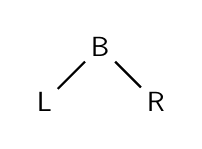
\begin{tikzpicture}
    \node (top) at (0,0) {$\mathsf{B}$};
    \node [below left  of=top] (left)  {$\mathsf{L}$};
    \node [below right of=top] (right) {$\mathsf{R}$};

    % Now draw the lines:
    \draw [thick, shorten <=-2pt, shorten >=-2pt] (top) -- (left);
    \draw [thick, shorten <=-2pt, shorten >=-2pt] (top) -- (right);
\end{tikzpicture}
\end{center}
Note that the points of $\BCover$ always have maxima with respect to specialization order, meaning that it is always possible to nondeterministically join points of $\BCover$ together.

We can arbitrarily think of $\mathsf{Left}$ as ``true'' and $\mathsf{Right}$ as ``false,'' which leads to a notion of order of binary covers in terms of degree of truth, where for $f, g : \Gamma \cto \BCover$, we say $f \leqq g$ if $f_*(\Img{\mathsf{Left}}) \le g_*(\Img{\mathsf{Left}})$ and $g_*(\Img{\mathsf{Right}}) \le f_*(\Img{\mathsf{Right}})$. Then binary covers form a De Morgan algebra with respect to this order; the corresponding conjunction, disjunction, and negation of $\BCover$s operations are continuous maps:
\begin{align*}
\cdot \wedge \cdot &: \BCover \times \BCover \cto \BCover
\\ x \wedge y &\triangleq \mathsf{cases}(x, y)
\begin{cases}
\mathsf{Left}(\wildcard), \mathsf{Left}(\wildcard)
 \quad &\Branch \quad
 \mathsf{L}
\\
\mathsf{Right}(\wildcard), \wildcard
 \quad &\Branch \quad
 \mathsf{R}
\\
\wildcard, \mathsf{Right}(\wildcard)
 \quad &\Branch \quad
 \mathsf{R}
\end{cases}
\\
\cdot \vee \cdot &: \BCover \times \BCover \cto \BCover
\\ x \vee y &\triangleq \mathsf{cases}(x, y)
\begin{cases}
\mathsf{Left}(\wildcard), \wildcard
 \quad &\Branch \quad
 \mathsf{L}
\\
\wildcard, \mathsf{Left}(\wildcard)
 \quad &\Branch \quad
 \mathsf{L}
\\
 \mathsf{Right}(\wildcard), \mathsf{Right}(\wildcard)
 \quad &\Branch \quad
 \mathsf{R}
\end{cases}
\\
\neg &: \BCover \cto \BCover
\\ \neg x &\triangleq \mathsf{cases}(x)
\begin{cases}
\mathsf{Left}(\wildcard)
 \quad &\Branch \quad
 \mathsf{R}
\\
\mathsf{Right}(\wildcard)
 \quad &\Branch \quad
 \mathsf{L}
\end{cases}.
\end{align*}

Since the output space is $\BCover$ where any two points have maxima, the gluing condition is trivially satisfied. We confirm by inspection that the patterns in the definitions of conjunction and disjunction are indeed covering.

One can confirm that the definitions of conjunction, disjunction, and negation indeed compute meets, joins, and De Morgan involution with respect to the $\leqq$ ordering.

\subsection{Alternative understandings of binary covers}

There are several other interpretations of binary covers that help explain why the two opens in a binary cover get ``opposite'' treatments in the definitions of conjunction and disjunction. Rather than thinking of a binary cover of $A$ as two opens $P, Q : \Open{A}$ such that (informally) $A \subseteq P \cup Q$, we can instead think of it as an open set $P$ and a \emph{closed} set $\overline{Q}$ which is the ``set-theoretic'' complement of $Q$, since the complement of an open set is closed. Then the fact that $(P, Q)$ is a binary cover means that $\overline{Q} \subseteq P$. Then conjunction computes intersections of the open and closed subspaces, while disjunction computes unions.
For instance, one can find the union of two closed sets by taking their complement to produce two open sets, taking the intersection of that, and then taking the complement to return to a closed set. Since we are simply ``encoding'' closed sets with their open complements, computing the ``union'' of closed subspaces just corresponds to taking an intersection of their open representatives.

\grammar{This} elicits the view of binary covers as ``approximate'' predicates, sandwiching a closed subspace inside an open one, with wiggle room for points in between. Any points in $\overline{Q}$ (and thus also $P$) will definitely compute to $\mathsf{Left}$, while any points outside of $P$ (and thus also outside $\overline{Q}$) will definitely compute to $\mathsf{Right}$, while in-between points, which are in $P$ but not $\overline{Q}$, are allowed to compute either way.

Finally, note that there is a homeomorphism $\BCover \cong \PLower^+(\bool)$ given by
\begin{align*}
\mathsf{to} &: \BCover \cto \PLower^+(\bool)
\\ \mathsf{to}(x) &\triangleq
  \mathsf{cases}(x)
  \begin{cases}
\mathsf{Left}(\wildcard)
 \quad &\Branch \quad
 \{ \btrue \}
\\
\mathsf{Right}(\wildcard)
 \quad &\Branch \quad
 \{ \bfalse \}
  \end{cases}
\\
\mathsf{from} &: \PLower^+(\bool) \cto \BCover
\\ \mathsf{from}(s) &\triangleq
  \mathsf{cases}(s)
  \begin{cases}
 \oincl{\lozenge(\cdot = \btrue)}{\wildcard}
 \quad &\Branch \quad
 \mathsf{L}
\\
 \oincl{\lozenge(\cdot = \bfalse)}{\wildcard}
 \quad &\Branch \quad
 \mathsf{R}
  \end{cases},
\end{align*}
which gives another understanding of binary covers, as representing nondeterministic truth values in Boolean logic. All of the logical operations defined for binary covers might make more sense when interpreted by the homeomorphism above. For instance, the conjunction operation on Boolean values,
$\&\& : \bool \times \bool \cto \bool$, can be lifted to a function of type $\PLower^+(\bool) \times \PLower^+(\bool) \cto \PLower^+(\bool)$ which applies $\&\&$ to its nondeterministic input possibilities and collects all the possible results. This lifted $\&\&$ operation, when translated by the above homeomorphism to $\BCover$, is identical to the $\wedge$ operation on $\BCover$s. \grammar{This} applies similarly to the other logical connectives that were defined on $\BCover$s.

Viewing the definitions in this manner easily confirms that the logical connectives defined for $\BCover$s give it the structure of a De Morgan algebra.
The specialization order on $\BCover$s corresponds to subset inclusion on $\PLower^+(\bool)$.

\subsection{Quantification over compact/overt spaces}

When working with sets, if a predicate $P$ on a set $A$ is decidable and if $A$ is Kuratowski-finite, then $\forall a : A.\ P(a)$ and $\exists a : A.\ P(a)$ are decidable as well. The analog of the finite sets in \textbf{Spc} are the compact/overt spaces.

\note{Perhaps I should re-do this to use the Vietoris powerspace of compact/overt subspaces of a given space. That way I can share the $\square, \lozenge$ notation with the lower powerspaces, and hopefully require fewer definitions.}
\note{cite nLab?}
A space $A$ is \emph{compact} if for every space $\Gamma$ and every open $U : \Open{\Gamma \times A}$, there is an open $\forall_A U : \Open{\Gamma}$ such that for every $V : \Open{\Gamma},$
\[
V \le_\Gamma \forall_A U \qquad \Leftrightarrow \qquad \top_A \times V \le_{\Gamma \times A} U.
\]
Similarly, a space $A$ is \emph{overt} if for every space $\Gamma$ and every open $U : \Open{\Gamma \times A}$, there is an open $\exists_A U : \Open{\Gamma}$ such that for every $V : \Open{\Gamma},$
\[
\exists_A U \le_\Gamma V  \qquad \Leftrightarrow \qquad U  \le_{\Gamma \times A} \top_A \times V.
\]

Note that for any space $A$, the points of $\PLower(A)$ correspond to overt subspaces of $A$.

These conditions are the definitions of universal and existential quantification in terms of adjoints, viewing $\Gamma$ as some context and opens as truth values in a context.

\begin{definition}
A \emph{compact/overt} space is a space $A$ that is both compact and overt, as well as satisfying an additional property, that says for all $\Gamma$ and all $P, Q : \Open{\Gamma \times A}$, we have
\begin{align*}
\forall_A(P \vee Q) &\le_\Gamma \forall_A P \vee \exists_A Q
\\  \forall_A P \wedge \exists_A Q &\le_\Gamma \exists_A (P \wedge Q).
\end{align*}
\end{definition}
These properties allow us to quantify over compact/overt spaces. Suppose we have a binary cover $f : \Gamma \times A \cto \BCover$ over a compact/overt space $A$ (in some context $\Gamma$). We define its universal quantification
\begin{align*}
\forall_A f &: \Gamma \cto \BCover
\\ \forall_A f(\gamma) &\triangleq \mathsf{cases}(\mathsf{\gamma})
\begin{cases}
\oincl{\forall_A f_*(\Img{\mathsf{Left}})}{\wildcard} &\Branch \mathsf{L}
\\ \oincl{\exists_A f_*(\Img{\mathsf{Right}})}{\wildcard} &\Branch \mathsf{R}
\end{cases}
\end{align*}

We can confirm this pattern match is covering, i.e.,
\[
\top \le_\Gamma \forall_A f_*(\Img{\mathsf{Left}}) \vee \exists_A f_*(\Img{\mathsf{Right}}),
\]
with the derivation
\begin{align*}
\top_\Gamma 
  &\le \forall_A (\top_A) \tag{$\forall_A$ adjointness}
\\ &\le \forall_A (f_*(\top_\BCover)) \tag{$f_*$ preserves $\top$}
\\ &\le \forall_A (f_*(\Img{\mathsf{Left}} \vee \Img{\mathsf{Right}}))
\\ &\le \forall_A(f_*(\Img{\mathsf{Left}}) \vee f_*(\Img{\mathsf{Right}}))  \tag{$f_*$ preserves joins}
\\ &\le \forall_A f_*(\Img{\mathsf{Left}}) \vee \exists_A f_*(\Img{\mathsf{Right}}) \tag{$A$ is compact/overt}.
\end{align*}

We can define $\exists_A f : \Gamma \cto \BCover$ by composing $\forall_A f$ with negation of binary covers.

\note{Consider removing this paragraph} If we expand to work in the gros topos, where we have higher-order functions, these functions for quantification, which allow us to extend quantification over opens to quantification over $\BCover$s, give us the operations $\forall_A : (A \to \BCover) \to \BCover$ and $\exists_A : (A \to \BCover) \to \BCover$ if $A$ is compact/overt.\footnote{Note that if $A$ is only compact or only overt, neither are possible, since the ``opposite'' quantification is used on the ``right'' side.}

Compact/overt spaces form a convenient class of spaces over which exhaustive reasoning is possible. The continuous image of a compact/overt space is compact/overt (similar to the fact that the image of a finite set under any map is finite). Like Kuratowski-finite subsets, compact/overt subspaces are closed under finite union, but not necessarily intersection.

For the real numbers, we have that for any real numbers $a, b : \R$ such that $a < b$, the closed interval from $a$ to $b$ is compact/overt. Of course, we can then take unions of intervals and still have compact/overt subspaces.

\subsection{Binary covers on $\R$}

We can define binary covers that give approximate order comparisons on $\R$ by defining, for each $\varepsilon : \rat^+$,\footnote{The lambda notation describes opens via the bijective correspondence between opens $U : \Open{A}$ and continuous maps $\chi_U : A \cto \Sigma$.}
\begin{align*}
[ \cdot < \cdot ]_\varepsilon &: \R \times \R \cto \BCover
\\ [x < y]_\varepsilon &\triangleq \mathsf{cases}(x, y)
\begin{cases}
\oincl{\lambda (x, y). x < y}{\wildcard} &\Branch \mathsf{L}
\\ \oincl{\lambda (x, y). x > y - \varepsilon}{\wildcard} &\Branch \mathsf{R}.
\end{cases}
\end{align*}

We can use \grammar{this} to query whether an arbitrary continuous map $f : \R \cto \R$ has no points that are close to being roots on a closed interval $[a, b]$, with the binary cover
\begin{align*}
\mathsf{no\_roots}_{\varepsilon} &: \One \cto \BCover
\\ \mathsf{no\_roots}_\varepsilon &\triangleq
  \forall_{[a,b]}(\lambda x. [ 0 < |f(x)| ]_\varepsilon)
\end{align*}
If we observe $\mathsf{Left}$ of the result, then indeed $f$ has no roots, while if we observe $\mathsf{Right}$ of the result, then there is some $x \in [a, b]$ such that $|f(x)| < \varepsilon$. Perhaps we have two maps $f, g : \R \times \R \cto \R$ and wish to confirm that there is some $x \in [0,1]$ such that for every $y \in [0,1]$, $f(x, y)$ is positive while $g(x,y)$ is negative:
\begin{align*}
\mathsf{apart}_{\varepsilon} &: \One \cto \BCover
\\ \mathsf{apart}_\varepsilon &\triangleq
  \exists_{[0,1]}(\lambda x. \forall_{[a,b]}(\lambda y. [ 0 < f(x, y) ]_\varepsilon \wedge [g(x, y) < 0]_\varepsilon)).
\end{align*}
Again, such a query has only false negatives (and its negation has only false positives). If we observe $\mathsf{Left}$, then it is certainly true, while if we observe $\mathsf{Right}$, then for every $x \in [0,1]$ there is a $y \in [0,1]$ such that either $f(x, y) < \varepsilon$ or $g(x, y) > -\varepsilon$.

\section{Related work}

\subsection{Alternative theories of constructive topology}

Synthetic topology gives an alternative computable interpretation of topology that differs subtly from formal topology and locale theory\cite{escardo2004, lesnik}. We will only describe synthetic topology informally, to take advantage of the alternative intuition it provides. In this understanding, data types from a (functional) programming language serve as spaces, and open sets are semidecidable predicates that take values of some type as arguments; for points in the open set, the semidecider must halt, whereas for points in the closed complement, the semidecider should not halt.

In this case, an open cover $U \le \bigvee_{i : I} V_i$ means that whenever $U$ halts, then some semidecider $V_i$ also halts.

This interpretation is limited to spatial locales (locales that also make sense as classical topological spaces), and covers indexed by countable sets. But it gives an alternative computational manner in which overlapping pattern matches could be achieved: run the semideciders for each case in the pattern match \emph{concurrently}. Since the cases must cover the entire space, the semidecider for one case will eventually halt, and at that point, proceed into the branch corresponding to that case.

\subsection{Pattern matching}

\cite{coquand1992} gives a topologically motivated explanation of pattern matching for dependently typed functional programming, describing patterns as (disjoint) partitions of a space.

\cite{dijkstra} introduces ``guarded commands,'' a language construct for imperative programming languages, where a branch can be chosen from a list of statements each guarded by a Boolean expression. Unlike in this work, each case in \cite{dijkstra} must be decidable.

\subsection{Binary covers}

Some of the modified Boolean spaces give topological interpretations of well-known fuzzy logics: $\bool_\bot$ corresponds to Kleene's three-valued logic, $\BCover \cong \PLower^+(\bool)$ to Priest's logic of paradox, and $\PLower(\bool)$ to Dunn/Belnap's four-valued logic \note{Cite them?}.

dReal is a tool that allows computation of approximate truth values over the real numbers \cite{dReal}, allowing order comparisons and bounded quantifiers. The calculus of binary covers presented here, when restricted to $\R$, provides similar computational abilities, but with a different foundational framework. In a sense, it shows how it is possible to generalize the theory behind dReal to general topological spaces.

\section{Discussion and conclusion}

We defined predicative locales and formal topologies in the Coq proof assistant and implemented the core pattern-matching construction (theorem \ref{pattern}). We also defined a function that, given any point $x$ of a space $A$, and any open cover $\top \le \bigvee_{i : I} U_i$ of $A$, returns an index $i : I$ such that $x \models U_i$. Executing this function allows computation of results from running continuous functions. The source code is submitted with this paper.

The programs described in this paper conceivably support reasonably efficient implementations, thanks to their use of formal topology and (predicative) locale theory, rather than a topology framework based on semidecision procedures. In the former frameworks, proofs of the validity of continuous maps defined by their inverse image maps not only confirm correctness but also provide the computational content.

Overlapping pattern matches seem useful for a variety of purposes, but in particular highlight the  importance of nondeterminism in constructing programs over spaces. The approximate root-finding procedure in the introduction and the case study of binary covers demonstrate useful nondeterministic programs that can be constructed with overlapping patterns.

A possible direction of future work would be to extend overlapping patterns to the gros topos $\mathcal{E}$ over \textbf{FSpc} (with the previously described open cover topology). For instance, we might want to have an overlapping pattern match that nondeterministically returns a \emph{function}, rather than simply a point of a space. Since \textbf{Spc} lacks exponentials in general, making sense of \grammar{this} would require extending the constructs defined here to $\mathcal{E}$.


% conference papers do not normally have an appendix


% use section* for acknowledgment
%\section*{Acknowledgment}
%The authors would like to thank...





% trigger a \newpage just before the given reference
% number - used to balance the columns on the last page
% adjust value as needed - may need to be readjusted if
% the document is modified later
%\IEEEtriggeratref{8}
% The "triggered" command can be changed if desired:
%\IEEEtriggercmd{\enlargethispage{-5in}}

% references section

% can use a bibliography generated by BibTeX as a .bbl file
% BibTeX documentation can be easily obtained at:
% http://mirror.ctan.org/biblio/bibtex/contrib/doc/
% The IEEEtran BibTeX style support page is at:
% http://www.michaelshell.org/tex/ieeetran/bibtex/
%\bibliographystyle{IEEEtran}
% argument is your BibTeX string definitions and bibliography database(s)
%\bibliography{IEEEabrv,../bib/paper}
%
% <OR> manually copy in the resultant .bbl file
% set second argument of \begin to the number of references
% (used to reserve space for the reference number labels box)
\bibliographystyle{IEEEtran}
\bibliography{LICS}




% that's all folks
\end{document}


